\documentclass[aspectratio=169,x11names]{beamer}
\usetheme{Pittsburgh}
\usepackage{xcolor}
\usepackage[utf8]{inputenc}
\usepackage[german]{babel}
\usepackage{amsmath}
\usepackage{amsfonts}
\usepackage{amssymb}
\usepackage{graphicx}
\usepackage{multicol}
\usepackage{wrapfig}
\usepackage{hyperref}
\usepackage{tikz}
\usetikzlibrary{shapes,arrows,automata,positioning}

\author{Jonas Betzendahl}
\title{Blockchain Science Slam}

\beamertemplatenavigationsymbolsempty 

% For Footnotes without markers on the slide
% https://tex.stackexchange.com/questions/30720/footnote-without-a-marker
\newcommand\blfootnote[1]{%
  \begingroup
  \renewcommand\thefootnote{}\footnote{#1}%
  \addtocounter{footnote}{-1}%
  \endgroup
}

%src: https://tex.stackexchange.com/questions/34921/how-to-overlap-images-in-a-beamer-slide
\def\Put(#1,#2)#3{\leavevmode\makebox(0,0){\put(#1,#2){#3}}}

\begin{document}

%------------------------------------------------------------------------------------
\section{Introduction}

\begin{frame}
\begin{center}
\Large \glqq Blockchain\grqq
\normalsize 

(Ein kurzer Input zum neuesten Hype)
\bigskip\bigskip

\Large Jonas Betzendahl\\
\texttt{@jbetzend}
\smallskip

\href{https://twitter.com/jbetzend}{
\includegraphics[scale=0.125]{images/twitter_logo.png}}
\href{https://github.com/lambdaTotoro}{
\includegraphics[scale=0.125]{images/github_logo.png}}
\href{https://whispeer.de/en/user/jbetzend}{
\includegraphics[scale=0.125]{images/whispeer_logo.png}}
\end{center}
\end{frame}

%--------------------------------------------------------------------------------------------------------------

\begin{frame}
\frametitle{Blockchain: The Hype is Real!}
 \Put(0,-100){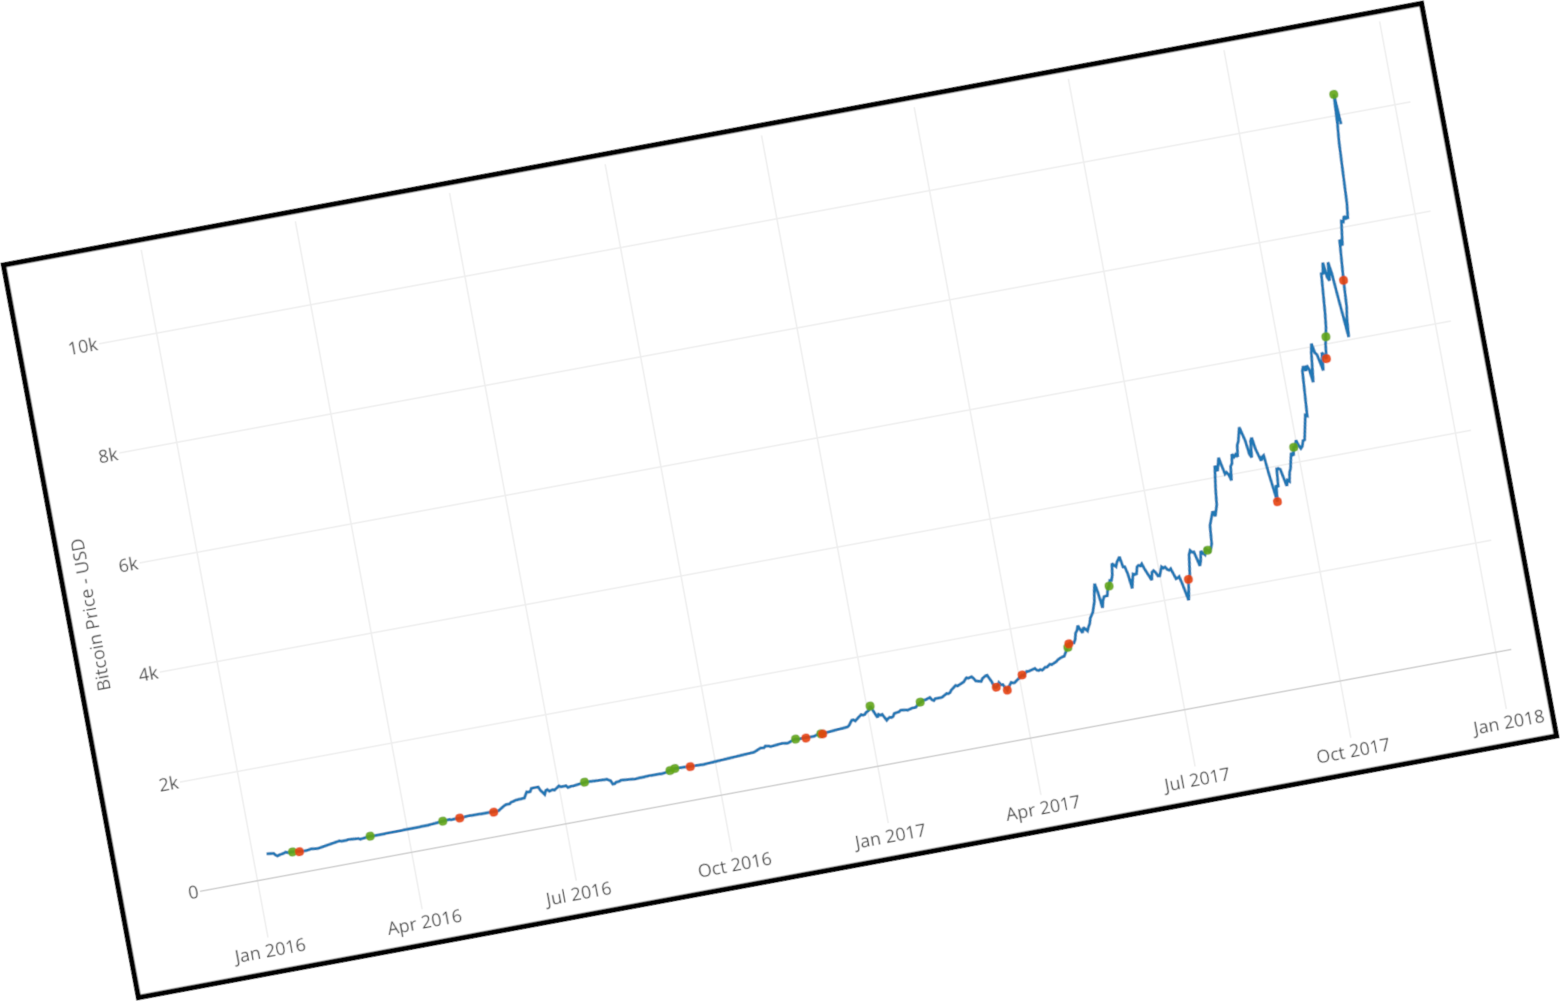
\includegraphics[scale=0.7]{images/exponential}}
 \Put(250,-100){
\includegraphics[scale=0.4]{images/bitcoin_gold}}
 \pause \Put(100,-100){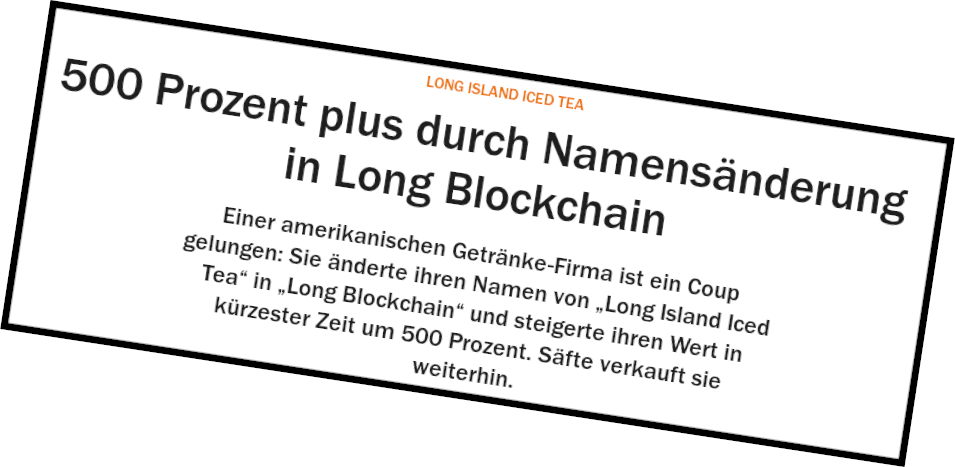
\includegraphics[scale=1]{images/saftladen}}
\pause \Put(30,80){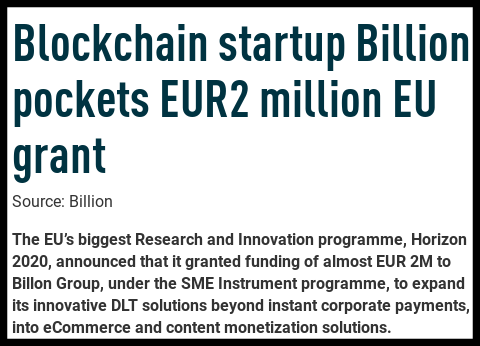
\includegraphics[scale=1]{images/funding}}
\pause \Put(100,-150){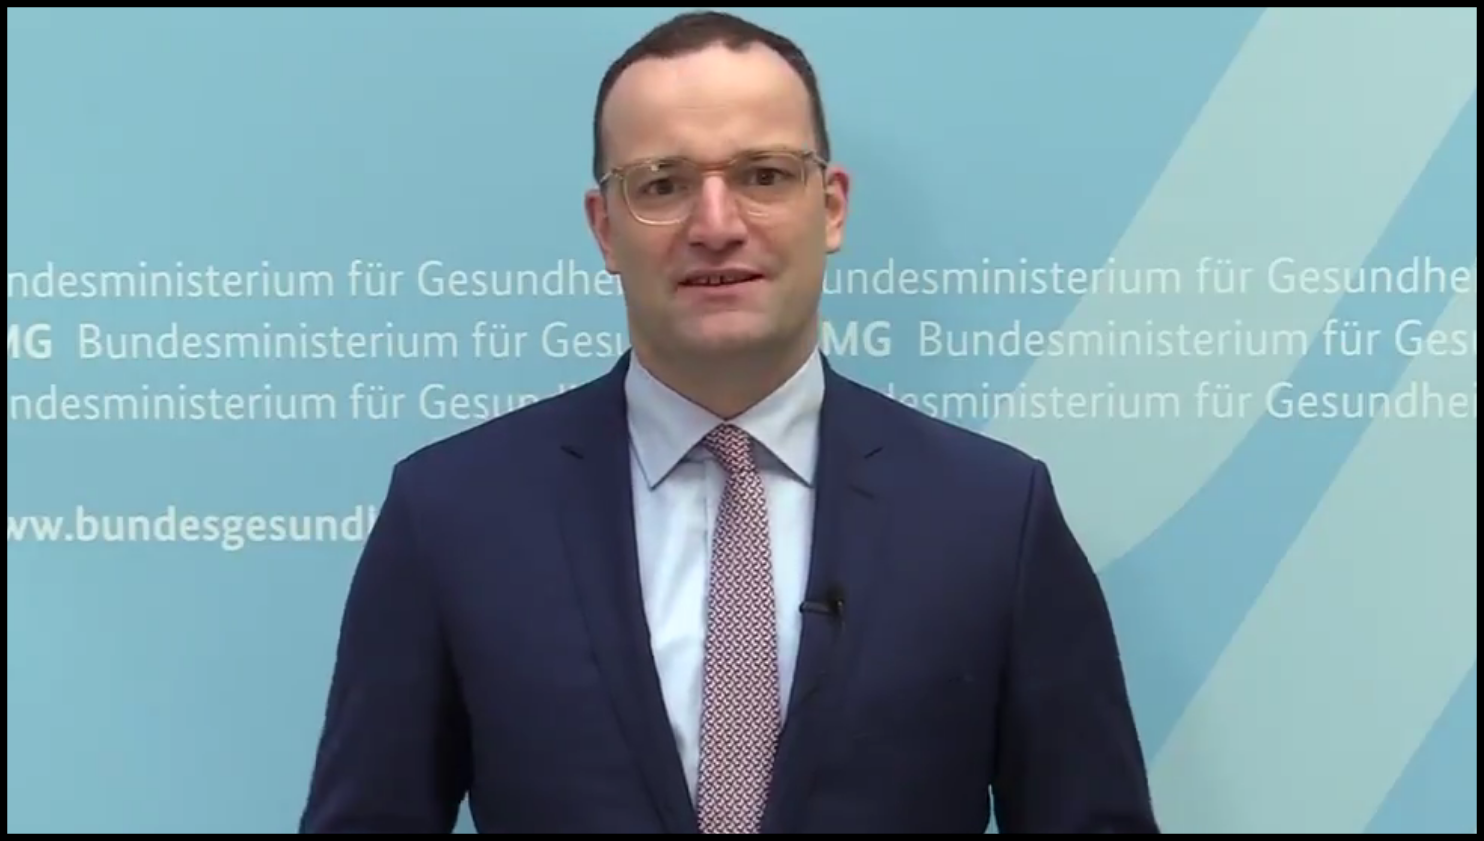
\includegraphics[scale=0.65]{images/spahn}}

\end{frame}

%--------------------------------------------------------------------------------------------------------------

\begin{frame}
\frametitle{Wie funktioniert so eine \glqq Blockchain\grqq ? (1)}

\tikzstyle{miner} = [rectangle, draw, fill=gray!20, 
    text width=5em, text centered, rounded corners, minimum height=4em]

    \begin{center}

\begin{multicols}{2}
\hspace*{40pt}
    \begin{tikzpicture}[font=\sffamily]
        % Setup the style for the states
        \tikzset{node style/.style={state, 
                                    minimum width=1.5cm,
                                    line width=1mm,
                                    fill=gray!20!white}}
 
        % Draw the states
        \node[node style] at (0, 0)     (bull)     {$P_1$};
        \node[node style] at (5, 0)     (bear)     {$P_2$};
        \node[node style] at (2.5, -4.2) (stagnant) {$P_3$};
 
        % Connect the states with arrows
        \draw[every loop,
              auto=right,
              line width=1mm,
              >=latex,
              draw=orange,
              fill=orange]
            (bull)     edge[bend right=20]            node {} (stagnant)
            (bull)     edge[bend right=20, auto=left] node {} (bear)
            (bear)     edge[bend right=20]            node {} (bull)
            (bear)     edge[bend right=20, auto=left] node {} (stagnant)
            (stagnant) edge[bend right=20]            node {} (bear)
            (stagnant) edge[bend right=20, auto=left] node {} (bull);
\end{tikzpicture}
\columnbreak
\pause
\begin{tikzpicture}
\node [miner, minimum height=1.5cm, yshift=-0.5cm, minimum width=2cm] (m1) {Miner$_1$};
\node [miner, below of=m1, yshift=-1.5cm, minimum height=1.5cm, minimum width=2cm] (m2) {Miner$_2$};
\node [miner, below of=m2, yshift=-1.5cm, minimum height=1.5cm, minimum width=2cm] (m3) {Miner$_3$};
\end{tikzpicture}

\end{multicols}  
    \end{center}
\end{frame}

\begin{frame}
\frametitle{Wie funktioniert so eine \glqq Blockchain\grqq ? (2)}
\begin{center}
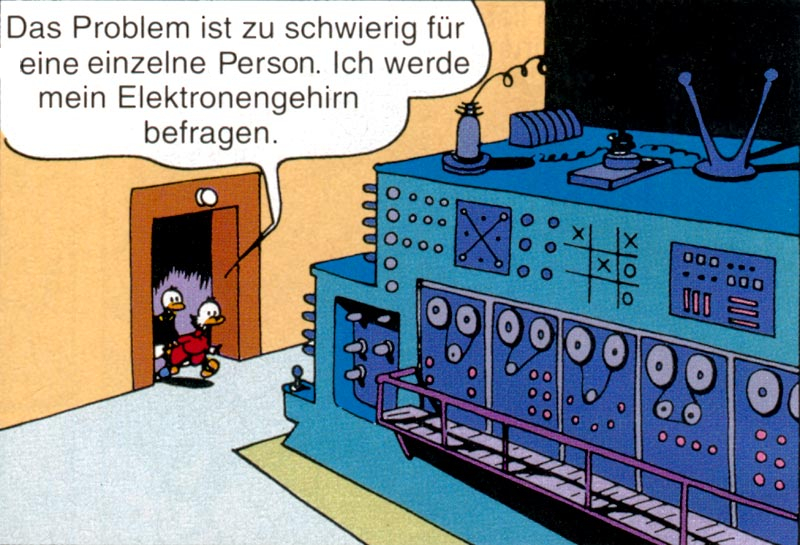
\includegraphics[scale=0.3]{images/elektronengehirn.jpg} 
\end{center}
\end{frame}

\begin{frame}
\frametitle{Wie funktioniert so eine \glqq Blockchain\grqq ? (3)}
\begin{center}
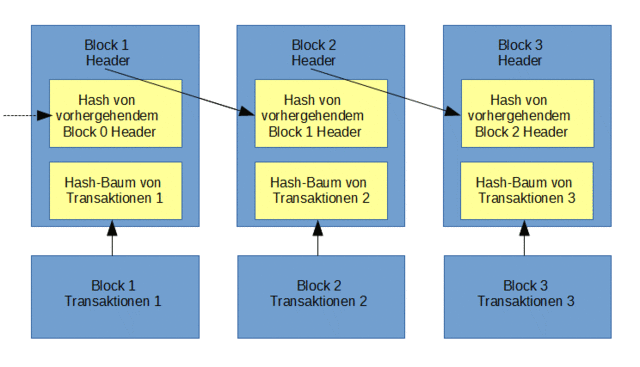
\includegraphics[scale=2]{images/BlockChain_D.png} 
\end{center}
\end{frame}

%--------------------------------------------------------------------------------------------------------------

\begin{frame}
\frametitle{Wann macht Blockchain Sinn?}

Eine Blockchain kommt unter Umständen in Frage, wenn ein Problem vorliegt, dass\dots
\bigskip

\begin{itemize}
\pause\item aus \emph{Transaktionen} besteht,
\pause\item diese eine \emph{totale Ordnung} brauchen,
\pause\item kein \emph{Vertrauen} zwischen Akteuren zulässt,
\pause\item nicht notwendigerweise gut \emph{skalieren} muss 
\end{itemize}
\end{frame}

%--------------------------------------------------------------------------------------------------------------

\begin{frame}
\frametitle{Probleme (1): Vertrauen}
Das Protokoll braucht kein Vertrauen, andere schon\dots\pause 
\bigskip\bigskip

\begin{center}

\includegraphics[scale=1]{images/mtgox.png} \qquad\qquad

\includegraphics[scale=0.15]{images/DAO-logo.png} 
\end{center}
\end{frame}

%--------------------------------------------------------------------------------------------------------------

\begin{frame}
\frametitle{Probleme (2): Skalierung}
Mining wird immer teurer\dots\pause

\begin{center}

\includegraphics[scale=2]{images/ireland.png} 
\pause \Put(-275,120){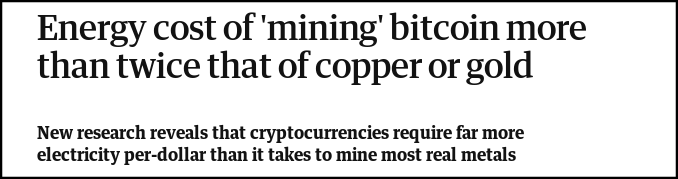
\includegraphics[scale=2]{images/mining_gold.png}}
\pause \Put(-275,120){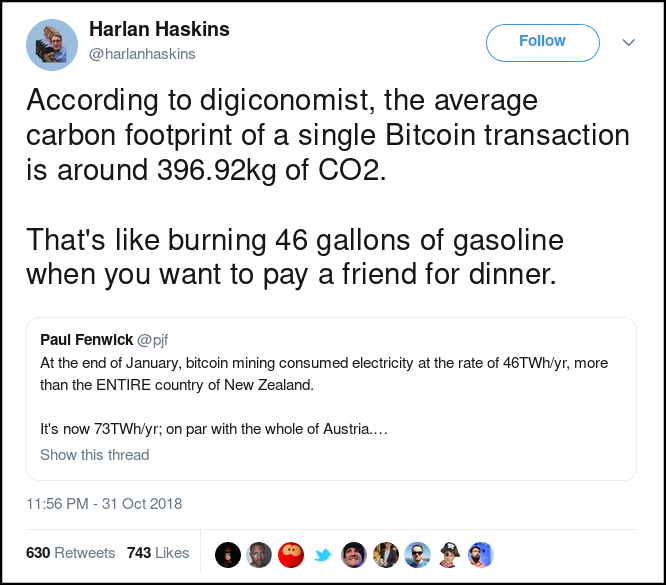
\includegraphics[scale=1.5]{images/co2.png}}
\end{center}
\end{frame}

%--------------------------------------------------------------------------------------------------------------

\begin{frame}
\frametitle{Probleme (3): You're doing it wrong!}

\begin{center}
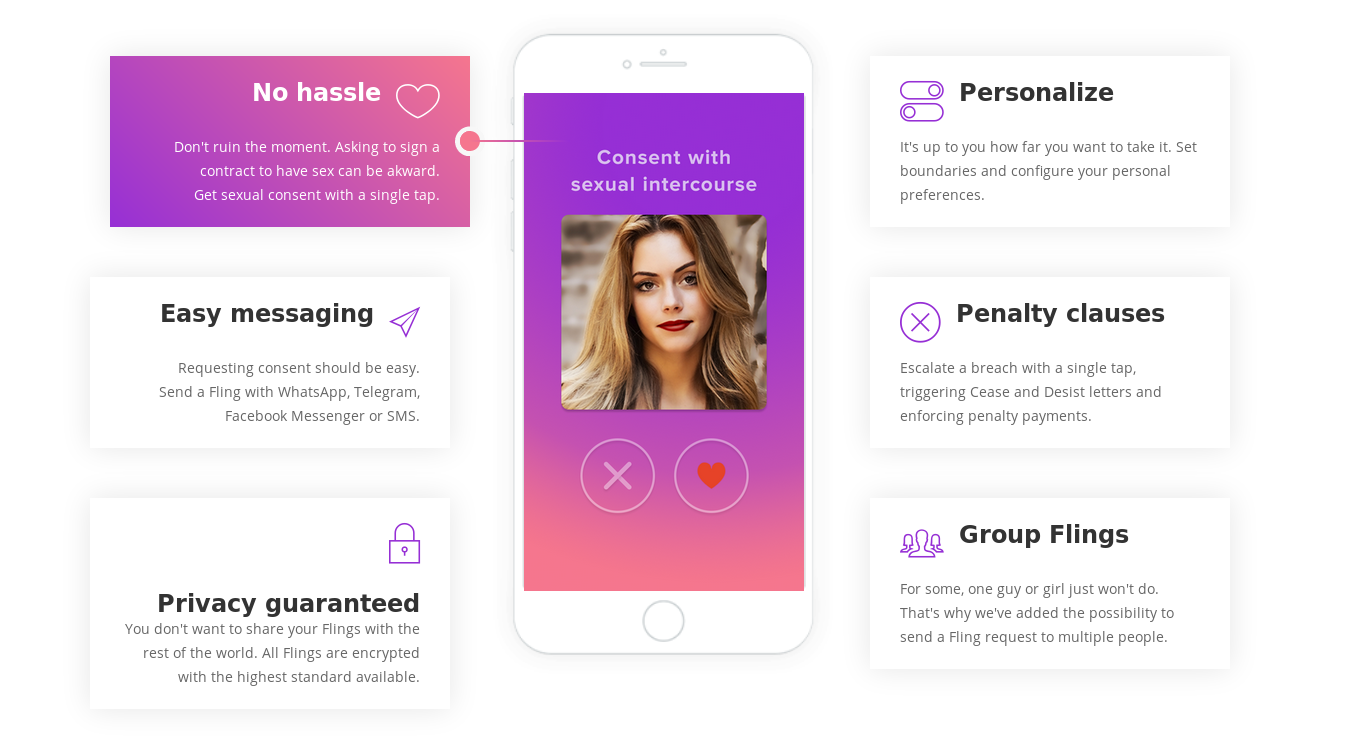
\includegraphics[scale=0.25]{images/consent_apps.png} 
\end{center}
\pause \Put(75,250){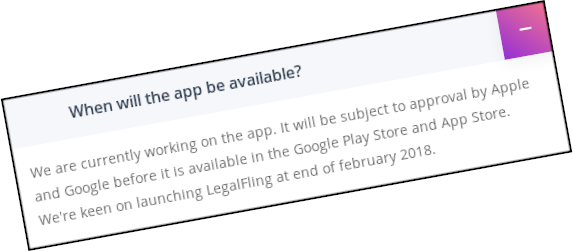
\includegraphics[scale=2]{images/launchdate.png}}
\end{frame}

%--------------------------------------------------------------------------------------------------------------

\begin{frame}
\frametitle{Brauche ich eine Blockchain?}
% Define block styles
\tikzstyle{decision} = [diamond, draw, fill=blue!20, 
    text width=4.5em, text badly centered, node distance=3cm, inner sep=0pt]
\tikzstyle{block} = [rectangle, draw, fill=blue!20, 
    text width=5em, text centered, rounded corners, minimum height=4em]
\tikzstyle{line} = [draw, -latex']
    
\begin{center}
\begin{tikzpicture}[ auto]
    % Place nodes
    \node [block, fill=green!40, minimum height=2cm, minimum width=3cm] (need) {Brauche ich eine\\ Blockchain?};
    \node [decision, right of=need,yshift=-0.5cm] (decideOne) {Trans-\\ aktional?};
    \node [decision, right of=decideOne, minimum height=2.35cm, minimum width=2.35cm, yshift=-1cm] (decideTwo) {Kein\\ Vertrauen?};
    \node [decision, right of=decideTwo, minimum height=2.35cm, minimum width=2.35cm, yshift=-2cm] (decideThree) {Skalierung\\ egal?};
    \node [block, below of=decideOne, fill=red!50, yshift=-2cm] (no) {Keine Blockchain!};
    \node [block, fill=red!25, above of=decideThree, minimum width=3cm, yshift=2.5cm] (stop) {Vielleicht\\ Blockchain?};
    % Draw edges
    \path [line] (need) -- (decideOne);
    \path [line] (decideOne) -- node {Nein} (no);
    \path [line] (decideTwo) -- node {Nein} (no);
    \path [line] (decideThree) -- node {Nein} (no);
    \path [line] (decideTwo) -- node {Ja} (decideThree);
    \path [line] (decideThree) -- node {Ja} (stop);
    \path [line] (decideOne) -- node [near start] {Ja} (decideTwo);
\end{tikzpicture}
\end{center}

\end{frame}

%--------------------------------------------------------------------------------------------------------------

\begin{frame}[fragile]
\begin{multicols}{2}

\vspace*{60pt}
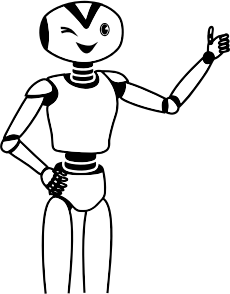
\includegraphics[scale=0.6]{images/Happy-Thumbs-Up-Robot.png} 

\columnbreak

\vspace*{60pt}

\Huge
\hspace*{-30pt}Vielen Dank für die\\ \hspace*{-20pt} Aufmerksamkeit!
\end{multicols}
\end{frame}

\end{document}

